\documentclass{article}
\usepackage{times}
\usepackage[utf8]{inputenc}
\usepackage[T1]{fontenc}
\usepackage[russian]{babel}
\usepackage[a4paper, total={6in, 8in}]{geometry}
\usepackage{dirtytalk}
\usepackage{graphicx}
\usepackage{hyperref}
\usepackage{listings}
\usepackage{color,soul}

\graphicspath{ {./img/} }

% code listings settings
\definecolor{lightgray}{rgb}{.9,.9,.9}
\definecolor{darkgray}{rgb}{.4,.4,.4}
\definecolor{purple}{rgb}{0.65, 0.12, 0.82}

\lstdefinelanguage{JavaScript}{
	keywords={break, case, catch, continue, debugger, default, delete, do, else, false, finally, for, function, if, in, instanceof, new, null, return, switch, this, throw, true, try, typeof, var, void, while, with},
	morecomment=[l]{//},
	morecomment=[s]{/*}{*/},
	morestring=[b]',
	morestring=[b]",
	ndkeywords={class, export, boolean, throw, implements, import, this},
	keywordstyle=\color{blue}\bfseries,
	ndkeywordstyle=\color{darkgray}\bfseries,
	identifierstyle=\color{black},
	commentstyle=\color{purple}\ttfamily,
	stringstyle=\color{red}\ttfamily,
	sensitive=true
}

\lstset{
	language=JavaScript,
	backgroundcolor=\color{lightgray},
	columns=fullflexible,
	basicstyle=\ttfamily,
	extendedchars=false,
	showstringspaces=false,
	showspaces=false,
	numbers=left,
	numberstyle=\footnotesize,
	numbersep=9pt,
	tabsize=2,
	breaklines=true,
	showtabs=false,
	captionpos=b
}


\begin{document}
\title{Лабораторная работа 2}

\date{\today}
\maketitle

\say{Сначала учите науку программирования и всю теорию. Далее выработаете свой программистский стиль. Затем забудьте все и просто программируйте.
— George Carrette}

\section{Введение}

Цель: изучить работу Ethereum, изучить Ganache


\section{Основные понятия}

\begin{itemize}
	\item Etheruim (эфир) -  платформа для создания децентрализованных онлайн-сервисов на базе блокчейна
	\item Smart Contract (умный контракт) - компьютерный алгоритм, предназначенный для заключения и поддержания коммерческих контрактов в технологии блокчейн. 	
\end{itemize}


Для выполнения лабораторной работы, необходимо восопльзоватся виртуальной машиной, на которой установлена Ubuntu 18.04 и весь необходимый набор ПО.

Теорию можно прочесть в файле Theory.pdf.

(Тут будет инфа о пути к тестовому проекту)


\section{Подготовка окружения}

Все необходимые зависимости уже установлены на виртуальную машину. Далее будут представлены необходимые программы и пакеты для выполнения лабораторной работы. 

\subsection{Ganache}

Ganache - это блокчейн для разработки Ethereum, которую вы можете использовать для развертывания контрактов, разработки приложений и запуска тестов. Он создает виртуальную цепочку Ethereum и генерирует некоторые поддельные учетные записи, которые мы будем использовать во время разработки (Рис. 1).

Для запуска Ganache, найдите значек в меню приложений. Сразу после запука будут установлены значения по умолчанию, контролирующие количество поддельных учетных записей и сумму ETH на их счетах.

\begin{figure}
    \centering
    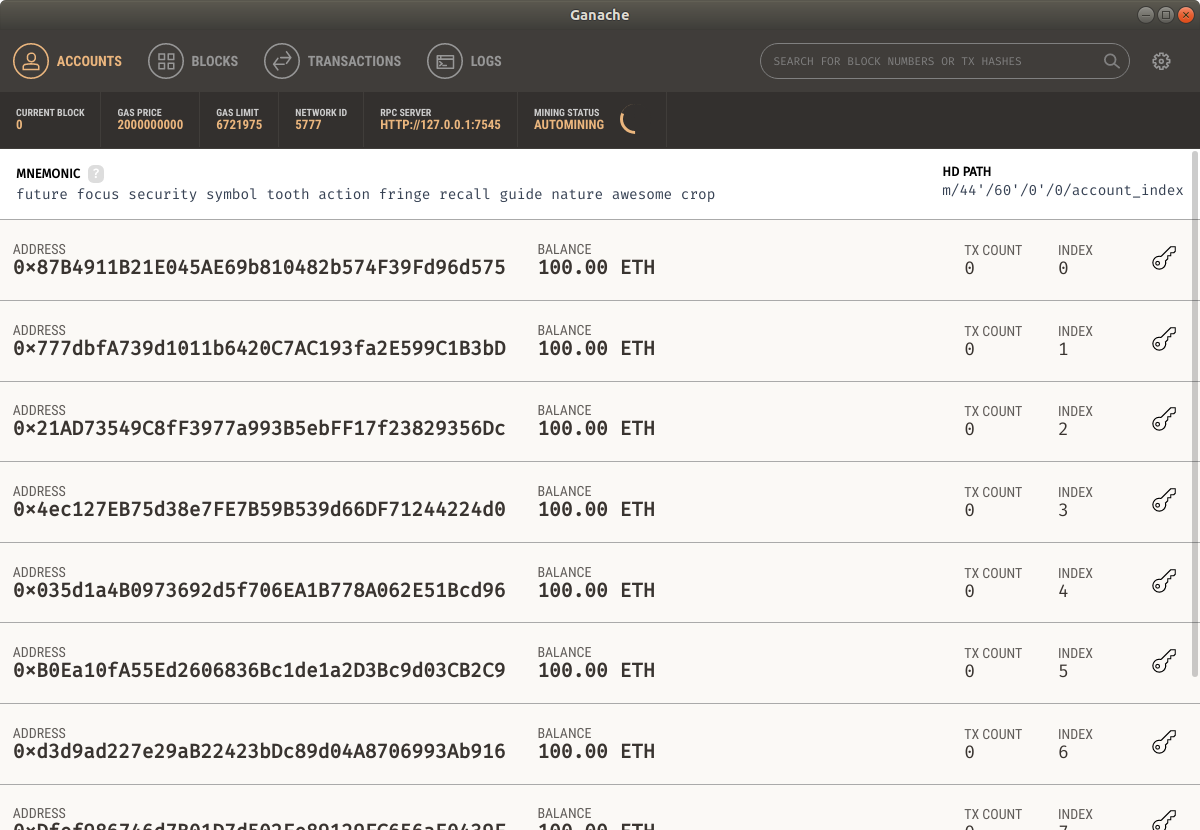
\includegraphics[scale=0.4]{ganache_1}
    \caption{Интерфейс Ganache.}
    \label{fig:ganache_1}
\end{figure}

\subsection{Metamask}

Metamask -  это криптовалютный кошелек, который встраивается в браузер Google Chrome и он нужен для упрощения передачи Эфира (Эфириум,  Ethereum, ETH)  или токенов ERC-20  в сети Эфириума. Мы будем использовать его для тестирования смарт-контрактов (Рис. 2).


\begin{figure}
    \centering
    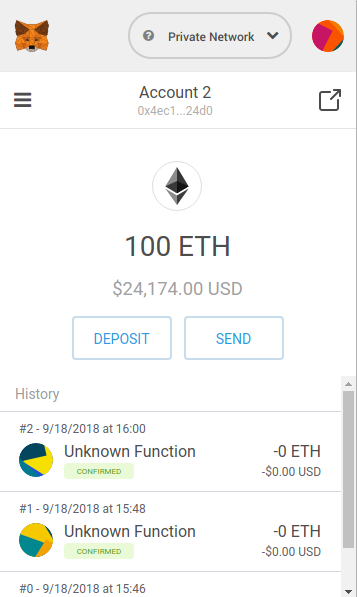
\includegraphics[scale=0.4]{metamask_1}
    \caption{Интерфейс MetaMask.}
    \label{fig:metamask_1}
\end{figure}


\subsection{Remix IDE}

Remix - это мощный инструмент с открытым исходным кодом, который помогает писать контракты Solidity прямо из браузера. Написанна на Javascript, Remix поддерживает как использование в браузере, так и локально (Рис. 3). Remix также поддерживает тестирование, отладку и развертывание смарт-контрактов и многое другое.

\begin{figure}
    \centering
    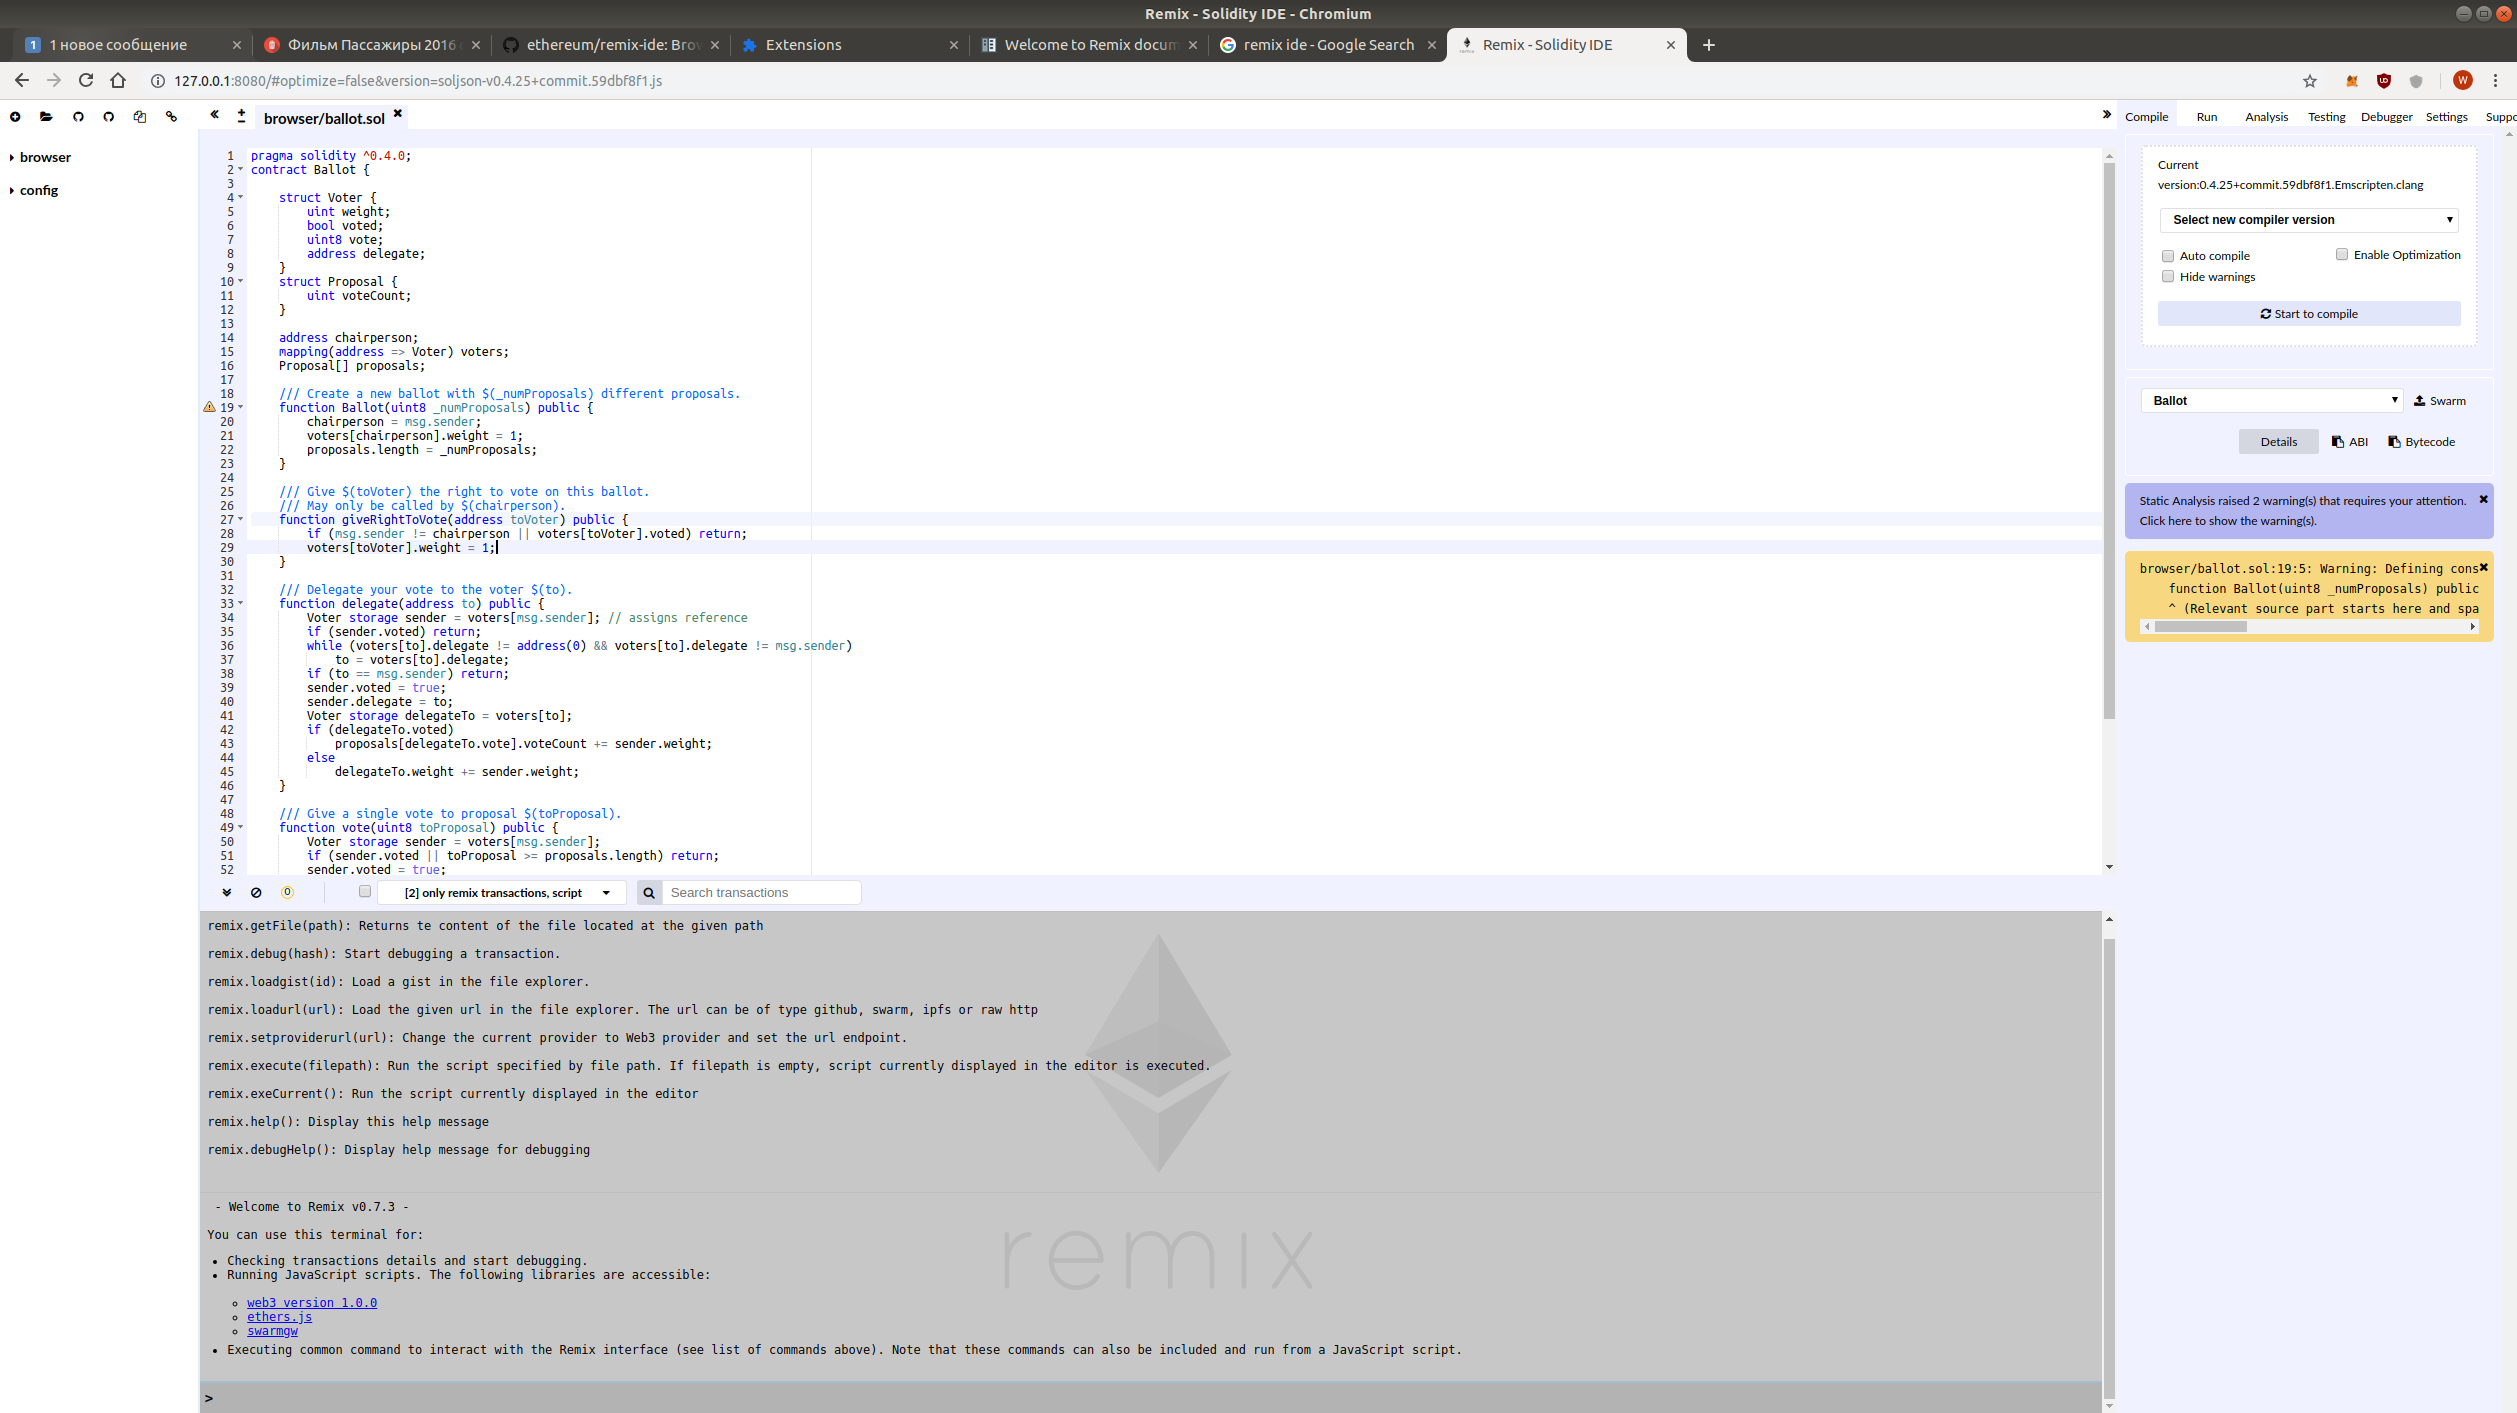
\includegraphics[scale=0.14]{remix_ide_1}
    \caption{Интерфейс Remix IDE.}
    \label{fig:remix_ide_1}
\end{figure}


На данный момент, она в некоторх моментах подтармаживает, и при работе на вирутальной машине, это вызывает дискомфорт, по этому советуется пользоватся VSCode, которая предустановлена на ВМ.

\section{Создание проекта}

Для выполнения лабораторной работы, воспользуемся уже готовым проектом, в нем будут необходимые файлы для фронтенда и т.п. Для скачивания тестового проекта, перейдите в каталог, куда будет скачан проект и выполнить:

\begin{lstlisting}[caption={Скачивание проекта pet-shop}]
$ truffle unbox pet-shop
\end{lstlisting}


После выполнения данной команды будет скачан проект в виде следующих файлов:

\begin{figure}
    \centering
    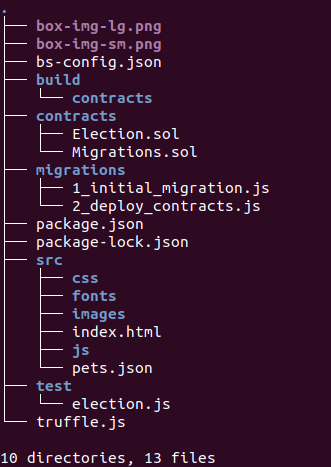
\includegraphics[scale=0.4]{project_tree}
    \caption{Дерево проекта.}
    \label{fig:project_tree}
\end{figure}


\begin{itemize}
	\item contracts:  Смарт-контракты. В папке уже есть контракт для миграций в блокчейн.
	\item migrations: Миграции. Эти миграции похожи на используемые в web фромеворках для изменения состояния базы данных.
	\item node modules: зависимости NodeJS.
	\item src: клиентские приложения.
	\item test: папка с тестами.
	\item truffle.js: файл с конфигурацией для truffle
\end{itemize}

\subsection{Создание первого смарт-контракта}
\medskip
Для создания смарт-контракта необходимо создать файл с расширением \hl{.sol} в папке \hl{contracts}. 
Пример:


\begin{lstlisting}[language=JavaScript, caption={contracts/Election.sol}]
pragma solidity 0.4.2;
contract Election {
	// Read/write candidate
	string public candidate;
	// Constructor
	function Election () public {
		candidate = "Candidate 1";
	}
}
\end{lstlisting}


Файл начинается с объявления версии solidity с помощью \hl{pragma}. Затем объявляем смарт-контракт с ключевым словом \hl{contract}, за которым следует название контракта. Затем мы объявляем переменную состояния, которая будет хранить значение имени кандидата. Переменные состояния позволяют нам записывать данные в блокчейн. Мы объявили, что эта переменная будет строкой, и мы установили ее видимость public. Поскольку она является public, solidity генерирует функцию getter, которая позволит получить доступ к этой переменной за пределами контракта.

Затем мы создаем функцию-конструктор, которая будет вызываться при каждом разворачивании смарт-контракта в цепочку. Здесь мы установим значение переменной состояния кандидата, которая будет сохранена в блокчейне после миграции. Обратите внимание, что функция конструктора имеет то же имя, что и смарт-контракт. Так solidity знает, что функция является конструктором.

\bigbreak

Теперь, когда мы создали основу для смарт-контракта, давайте посмотрим, можно ли его развернуть в блокчейн. Для этого нам нужно создать новый файл в каталоге миграции. Из корня проекта создайте новый файл из командной строки следующим образом:

\begin{lstlisting}[language=JavaScript, caption={contracts/Election.sol}]
var Election = artifacts.require("./Election.sol");

	module.exports = function(deployer) {
	deployer.deploy(Election);
};
\end{lstlisting}


После добавления новой миграции, ее нужно применить выполнив:

\begin{lstlisting}
$ truffle migrate
\end{lstlisting}

В консоли должно быть что то подобное:

\begin{lstlisting}
Compiling ./contracts/Election.sol...
Compiling ./contracts/Migrations.sol...
^----------------------^

Writing artifacts to ./build/contracts

Using network 'development'.

Running migration: 1_initial_migration.js
Deploying Migrations...
... 0x8c07a54c548ed49128b8fb2d17fa071b118019b6590536efd1fc2f0d49d3a850
Migrations: 0x24a632b41f13d45b189670ed3730ef610cb2bd29
Saving successful migration to network...
... 0x8c3023da63417b2debfcdeedefb78ca379aced324ac8d688335f7ce0dcfd37bc
Saving artifacts...
Running migration: 2_deploy_contracts.js
Deploying Election...
... 0xd53622e3735d4284f19b2b751913f251983e3f4163abb35daf1bb30a199c17df
Election: 0x850643f300b2516518d4c7b7f093e107957fcc17
Saving successful migration to network...
... 0xbafe0c2afb2fe2639500e8ba03e7b2fd13cda795cdabdad8f585bef2ab14cf59
Saving artifacts...
\end{lstlisting}

Можно протестировать в консоли, как работает наш модуль:


\begin{lstlisting}
$ truffle console
\end{lstlisting}

Создадим инстанс смарт-контракта и попробуем считать имя первого кандидата:

\begin{lstlisting}
>> Election.deployed().then(function(instance) { app = instance })
\end{lstlisting}

Сдесь \hl{Election} это имя переменной которая была создана в файле миграций.
Мы получили инстанс контракта из фунции \hl{deploted()}.

После этого, можно считать переменные:

\begin{lstlisting}
>> app.candidate()
	// => 'Candidate 1'
\end{lstlisting}


Вот и все, первый смарт-контракт готов!) Congratulations!



\begin{thebibliography}{9}

	\bibitem{lamport94}
	  \emph{Как работает Эфириум (Ethereum)?}
	  https://habr.com/post/407583/

\end{thebibliography}

\end{document}